\documentclass[11pt, a4paper]{article}
\usepackage[T1]{fontenc}
\usepackage[utf8]{inputenc}
\usepackage{geometry}
\geometry{verbose, tmargin=2cm, bmargin=2cm, lmargin=2cm, rmargin=2cm}
\usepackage{amsmath, amssymb, amsfonts}
\usepackage{graphicx}
\usepackage{caption}
\usepackage{subcaption}
\usepackage{hyperref}
\usepackage{float}
\usepackage{multirow}
\usepackage[numbers]{natbib}
\usepackage{array}
\usepackage{parskip} % Adds spacing between paragraphs and removes indentation

% Title and Author
\title{\textbf{Evaluating Multi-Dimensional Fitting Methods: Joint Maximum Likelihood vs Weighted \textit{sWeights} Fits}}
\author{
    Shahab Yousef-Nasiri (sy475) \\
    \small Department of Physics, University of Cambridge \\
    \small Word Count: 2982
}
\date{}

\begin{document}
\maketitle

% Abstract
\begin{abstract}
This study evaluates two fitting techniques for parameter estimation in a two-dimensional dataset; (1) a joint extended likelihood fit performed simultaneously across both variables \( X \) and \( Y \), and (2) a sequential weighted fit using \textit{sWeights}, which decouples the fitting process. The signal is modeled as a truncated Crystal Ball function in \( X \) and an exponential decay in \( Y \), alongside a background component. Using \texttt{iminuit}, extended likelihood fits were performed with well-defined parameter bounds and initial guesses for optimization. A parametric bootstrap study was conducted to assess the bias and uncertainty of the estimated decay constant \( \lambda \) using both techniques. The joint fit demonstrated negligible bias and reduced uncertainties as the sample size increased, leveraging the full two-dimensional information. Conversely, the \textit{sWeights} method, while computationally efficient, introduced a small positive bias due to its decoupling assumption. These findings highlight the trade-offs between precision, computational efficiency, and the treatment of multidimensional data in parameter estimation tasks.  
\end{abstract}

\newpage
\tableofcontents
\newpage
\section{Introduction}

The estimation of model parameters from experimental data is a foundational task in statistical modeling. In this study, we evaluate two fitting techniques for multi-dimensional likelihood estimation: a joint maximum likelihood fit that utilizes the full two-dimensional probability density function (PDF), and a sequential weighted fit using \textit{sWeights}, which decouples the fitting process into two stages. 

The model under investigation comprises a signal component and a background component in two dimensions, \( X \in [0, 5] \) and \( Y \in [0, 10] \). The signal is modeled using a truncated Crystal Ball distribution in \( X \) and an exponential decay in \( Y \). The background components are modeled by a uniform distribution in \( X \) and a truncated Gaussian distribution in \( Y \).
\subsection{Joint Probability Density Function}

The joint PDF for the signal and background components is expressed as:
\begin{equation}
    f(X, Y) = f_s \cdot g_s(X) h_s(Y) + (1 - f_s) \cdot g_b(X) h_b(Y),
\end{equation}
where:
\begin{itemize}
    \item \( f_s \): Signal fraction, defining the proportion of the total probability density attributed to the signal.
    \item \( g_s(X) \): The signal PDF in \( X \), defined by a truncated Crystal Ball distribution over \( [0, 5] \) (detailed in Section \ref{crystal_ball_section}).
    \item \( h_s(Y) \): The signal PDF in \( Y \), defined by an exponential decay truncated over \( [0, 10] \):
    \begin{equation}
        h_s(Y) = \frac{\lambda e^{-\lambda Y}}{1 - e^{-10 \lambda}}, \quad Y \in [0, 10],
    \end{equation}
    where the denominator \( 1 - e^{-10 \lambda} \) ensures proper normalization over the range.
    \item \( g_b(X) \): The background PDF in \( X \), modeled as a uniform distribution over \( [0, 5] \):
    \begin{equation}
        g_b(X) = \frac{1}{5}, \quad X \in [0, 5].
    \end{equation}
    \item \( h_b(Y) \): The background PDF in \( Y \), defined by a truncated Gaussian distribution with mean \(\mu_b\) and standard deviation \(\sigma_b\), over \( [0, 10] \):
    \begin{equation}
        h_b(Y) = \frac{1}{\sigma_b \sqrt{2\pi}} e^{-\frac{(Y - \mu_b)^2}{2\sigma_b^2}} \cdot \frac{1}{\Phi\left(\frac{10 - \mu_b}{\sigma_b}\right) - \Phi\left(\frac{0 - \mu_b}{\sigma_b}\right)},
    \end{equation}
    where \(\Phi(x)\) is the cumulative distribution function (CDF) of the standard normal distribution.
\end{itemize}
This formulation ensures proper normalization of the joint PDF over the truncated regions for both the signal and background components.

\subsection{Crystal Ball Probability Distribution \label{crystal_ball_section}}

The Crystal Ball distribution consists of a Gaussian core and a power-law tail. It is defined as:
\begin{equation}
    g_s(X; \mu, \sigma, \beta, m) = N \cdot \begin{cases} 
        e^{-Z^2 / 2}, & \text{for } Z > -\beta, \\
        \left( \frac{m}{\beta} \right)^m e^{-\beta^2 / 2} \left( \frac{m}{\beta} - \beta - Z \right)^{-m}, & \text{for } Z \leq -\beta,
    \end{cases}
\end{equation}
where:
\begin{itemize}
    \item \( Z = \frac{X - \mu}{\sigma} \): The normalized variable.
    \item \( \mu \): Location parameter, controlling the center of the Gaussian core.
    \item \( \sigma \): Scale parameter, determining the width of the Gaussian core.
    \item \( \beta \): Transition point between the Gaussian core and the power-law tail.
    \item \( m \): Slope of the power-law tail.
\end{itemize}
The distribution is valid for \( \beta > 0 \) and \( m > 1 \), ensuring a well-defined transition and finite normalization.
\subsubsection{Normalization Constant}

To ensure that the Crystal Ball PDF integrates to unity, the normalization constant \( N \) is derived from the following condition:
\[
\int_{-\infty}^\infty p(X; \mu, \sigma, \beta, m) dX = 1.
\]
Using the change of variable \( Z = \frac{X - \mu}{\sigma} \), we have \( dX = \sigma \, dZ \). Substituting this into the integral:
\[
\int_{-\infty}^\infty p(X; \mu, \sigma, \beta, m) dX = N \int_{-\infty}^\infty p(Z; \beta, m) \sigma \, dZ = 1.
\]
Rearranging for \( N \), the normalization constant is given by:
\begin{equation}
    N^{-1} = \sigma \int_{-\infty}^\infty p(Z; \beta, m) dZ.
    \label{eq:normalization_condition}
\end{equation}

\paragraph{Splitting the Integral:} The PDF \( p(Z; \beta, m) \) is piecewise-defined, allowing us to split the integral into two parts:
\begin{equation}
    N^{-1} = \sigma \left[ I_{\text{Gaussian}} + I_{\text{Power-law}} \right],
    \label{eq:split_integral}
\end{equation}
where:
\begin{itemize}
    \item \( I_{\text{Gaussian}} \) accounts for the Gaussian core (\( Z > -\beta \)).
    \item \( I_{\text{Power-law}} \) accounts for the power-law tail (\( Z \leq -\beta \)).
\end{itemize}

\paragraph{Gaussian Core Contribution:}
For \( Z > -\beta \), the Gaussian probability density function (PDF) simplifies to:
\[
p(Z; \beta, m) = e^{-Z^2 / 2}.
\]

To compute the contribution over the region \( Z \in [-\beta, \infty) \), we evaluate the integral:
\[
I_{\text{Gaussian}} = \int_{-\beta}^\infty e^{-Z^2 / 2} \, dZ.
\]

Using the property \( \Phi(-\beta) = 1 - \Phi(\beta) \), we find:
\[
I_{\text{Gaussian}} = \sqrt{2\pi} - \int_{-\infty}^{-\beta} e^{-Z^2 / 2} \, dZ \\
= \sqrt{2\pi} \Phi(\beta).
\]

Thus, the Gaussian core contribution is:
\begin{equation}
    I_{\text{Gaussian}} = \sqrt{2\pi} \Phi(\beta).
    \label{eq:gaussian_contribution}
\end{equation}

\paragraph{Power-Law Tail Contribution:}
For \( Z \leq -\beta \), the PDF is defined as:
\[
p(Z; \beta, m) = \left( \frac{m}{\beta} \right)^m e^{-\beta^2 / 2} \left( \frac{m}{\beta} - \beta - Z \right)^{-m}.
\]
Using the substitution \( u = \frac{m}{\beta} - \beta - Z \), such that \( dZ = -du \), the limits transform as:
\[
Z \to -\beta \implies u = \frac{m}{\beta}, \quad Z \to -\infty \implies u \to \infty.
\]
The integral becomes:
\[
I_{\text{Power-law}} = \int_{-\infty}^{-\beta} p(Z; \beta, m) dZ = \left( \frac{m}{\beta} \right)^m e^{-\beta^2 / 2} \int_{\infty}^{m / \beta} u^{-m} (-du).
\]

Evaluating the integral:
\[
\int_{m / \beta}^\infty u^{-m} du = \frac{u^{1-m}}{1-m} \bigg|_{m / \beta}^\infty = \frac{\left( \frac{m}{\beta} \right)^{1-m}}{m - 1}.
\]
Thus:
\begin{equation}
    I_{\text{Power-law}} = \frac{m}{\beta (m - 1)} e^{-\beta^2 / 2}.
    \label{eq:powerlaw_contribution}
\end{equation}

\paragraph{Combining Results:}
The normalization constant is:
\begin{equation}
    N^{-1} = \sigma \left[ \sqrt{2\pi} \Phi(\beta) + \frac{m}{\beta (m - 1)} e^{-\beta^2 / 2} \right].
    \label{eq:final_normalization_constant}
\end{equation}
This ensures the PDF is properly normalized over the entire domain.
\subsection{Distribution Plots}



To better understand the behavior of the model components, we present the marginal distributions in \(X\) and \(Y\), along with their respective signal and background components, in a single plot.
\begin{figure}[H]
    \centering
    \begin{subfigure}[b]{0.48\textwidth}
        \centering
        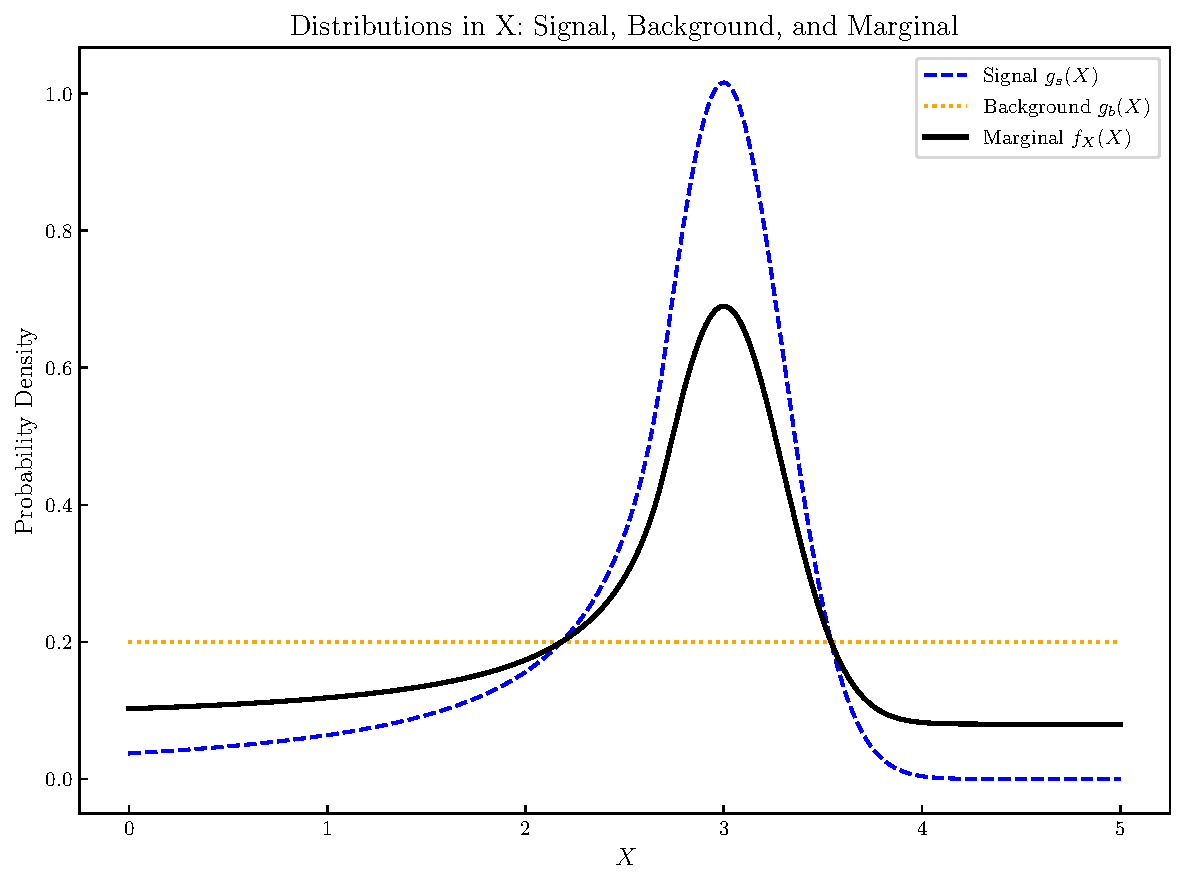
\includegraphics[width=\textwidth]{marginal_distribution_X.pdf}
        \caption{Marginal distribution in \(X\).}
        \label{fig:marginal_X}
    \end{subfigure}
    \hfill
    \begin{subfigure}[b]{0.48\textwidth}
        \centering
        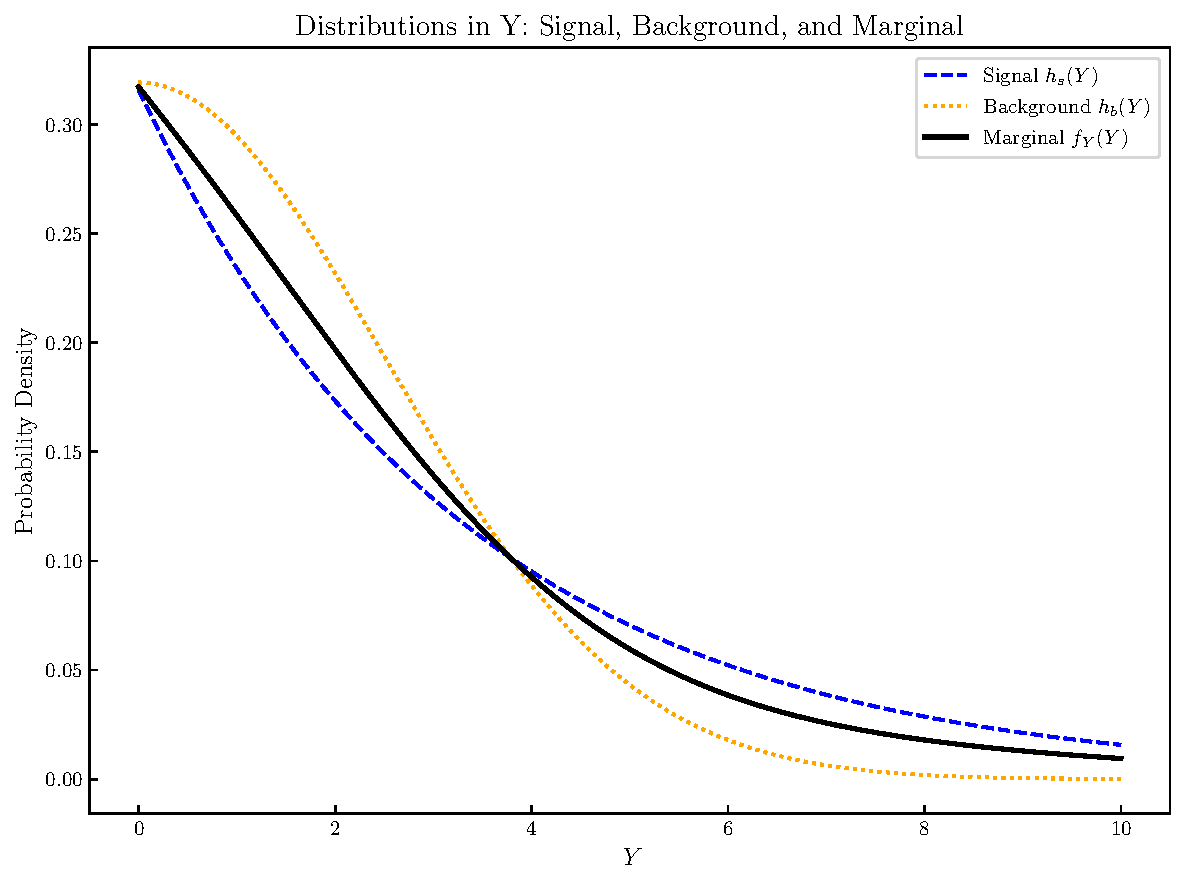
\includegraphics[width=\textwidth]{marginal_distribution_Y.pdf}
        \caption{Marginal distribution in \(Y\).}
        \label{fig:marginal_Y}
    \end{subfigure}
    \caption{Marginal distributions in \(X\) and \(Y\), showing their respective signal and background components.}
    \label{fig:marginal_distributions_split}
\end{figure}


\section{Methodology}
\subsection{Distributions}

Correct implementation of the probability density functions (PDFs) for the signal and background components in both dimensions is critical for ensuring computational efficiency and accuracy. The following techniques were employed in defining and implementing the distributions:

\paragraph{Precomputing Truncation Normalization Constant}
For the signal component in \( X \), the Crystal Ball distribution requires a truncation normalization constant to ensure the PDF integrates to unity over the truncated range. Instead of recalculating this constant during each evaluation, it is precomputed using numerical integration over the interval \( X \in [0, 5] \). This approach significantly reduces runtime computational overhead, especially when the PDF is evaluated repeatedly during sampling and fitting.

\paragraph{Vectorization and JIT Compilation}
All distributions were implemented using vectorized operations to handle arrays of inputs efficiently. The use of Just-In-Time (JIT) compilation via \texttt{Numba} further optimizes the evaluation of PDFs by compiling Python functions to machine code at runtime ~\cite{lam2015numba}. This combination ensures that PDF evaluations are both fast and scalable, even for large datasets.

\paragraph{Error Function Approximation}
For the truncated Gaussian background in \( Y \), the normalization constant involves the cumulative distribution function (CDF) of the Gaussian, which depends on the error function (\( \text{erf} \)). To ensure compatibility with JIT compilation and avoid incompatibilities with external libraries, an approximate error function (\( \text{erf} \)) was implemented using a polynomial expansion ~\cite{abramowitz1968handbook}. 


\paragraph{Normalization Testing}
To validate the correctness of the implementations, integrals of the PDFs were numerically computed over their respective domains. The results were checked to ensure they sum to unity, confirming that the normalization constants were correctly applied.
\subsection{Sampling Techniques}

The sampling process for generating data points is divided into two categories: signal and background.

\subsubsection{Signal Sampling}

Signal samples are drawn from \( g_s(X) \) (Crystal Ball distribution) and \( h_s(Y) \) (truncated exponential distribution). The sampling technique employed is \textbf{inverse transform sampling}, which involves~\cite{olver2013fast}:

\begin{enumerate}
    \item Compute the cumulative distribution function (CDF) of the target distribution.
    \item Generate uniform random numbers \( U \sim \text{Uniform}(0, 1) \).
    \item Map \( U \) to the CDF to obtain samples \( X \) by solving \( F(X) = U \). 
          For simple distributions, this inversion can be done analytically; for complex ones, numerical methods are employed.
\end{enumerate}

\paragraph{Sampling in \( Y \): Truncated Exponential Distribution}
For the truncated exponential distribution \( h_s(Y) \), the CDF is available in closed form:
\[
F(Y) = \frac{1 - e^{-\lambda_s Y}}{1 - e^{-\lambda_s \cdot 10}}, \quad Y \in [0, 10].
\]
The inverse of this CDF is given analytically as:
\[
Y = -\frac{\ln(1 - U \cdot (1 - e^{-\lambda_s \cdot 10}))}{\lambda_s}, \quad U \sim \text{Uniform}(0, 1).
\]
This direct inversion avoids numerical approximations and avoids the computational inefficiency of rejection sampling, guaranteeing exact samples from the truncated exponential distribution.

\paragraph{Sampling in \( X \): Truncated Crystal Ball Distribution}
The Crystal Ball distribution \( g_s(X) \), due to its more complex functional form, requires a numerical approach for sampling. The steps are as follows:
\begin{itemize}
    \item \textbf{Numerical CDF Construction}: The CDF is computed by numerically integrating the Crystal Ball PDF over a finely spaced grid of \( X \) values within the truncation bounds \( [0, 5] \). This is achieved using methods like the trapezoidal rule.
    \item \textbf{CDF Lookup via Interpolation}: To generate a sample \( X \), the following steps are performed:
\begin{enumerate}
    \item Generate a uniform random number \( U \sim \text{Uniform}(0, 1) \).
    \item Find two precomputed CDF values \( F(X_i) \) and \( F(X_{i+1}) \) such that:
    \[
    F(X_i) \leq U < F(X_{i+1}).
    \]
    \item Approximate the corresponding \( X \)-value using linear interpolation between \( X_i \) and \( X_{i+1} \):
    \[
    X = X_i + \frac{U - F(X_i)}{F(X_{i+1}) - F(X_i)} \cdot (X_{i+1} - X_i),
    \]
    where \( F(X_i) \) and \( F(X_{i+1}) \) are the cumulative probabilities at grid points \( X_i \) and \( X_{i+1} \), respectively.
\end{enumerate}

\end{itemize}

\subsubsection{Background Sampling}

Background samples are drawn from \( g_b(X) \) (uniform distribution) and \( h_b(Y) \) (truncated Gaussian distribution).

\paragraph{Sampling in \( X \): Uniform Distribution}
The uniform background distribution \( g_b(X) \) is straightforward to sample:
\[
X \sim \text{Uniform}(0, 5).
\]
This involves directly generating random numbers within the specified range.

\paragraph{Sampling in \( Y \): Truncated Gaussian Distribution}
The truncated Gaussian background \( h_b(Y) \) is also sampled using the inverse transform sampling method:

The \texttt{scipy.stats.truncnorm} library function is used, which  handles the truncation bounds \([0, 10]\).



\subsubsection{Combined Sampling}
The combined sampling process integrates signal and background components:
\begin{enumerate}
    \item Each sample is probabilistically assigned to either signal or background based on the signal fraction \( f_s \).
    \item Samples are then drawn from the corresponding distributions: \( g_s(X), h_s(Y) \) for the signal or \( g_b(X), h_b(Y) \) for the background.
\end{enumerate}

\subsubsection{Joint and Marginal Sampling Comparisons}

To validate the sampling techniques, the actual joint PDF and sampled joint data are visualized side by side, followed by individual marginal distributions for \( X \) and \( Y \) comparing actual and sampled distribution.

\begin{figure}[H]
    \centering
    \begin{subfigure}[b]{0.47\textwidth}
        \centering
        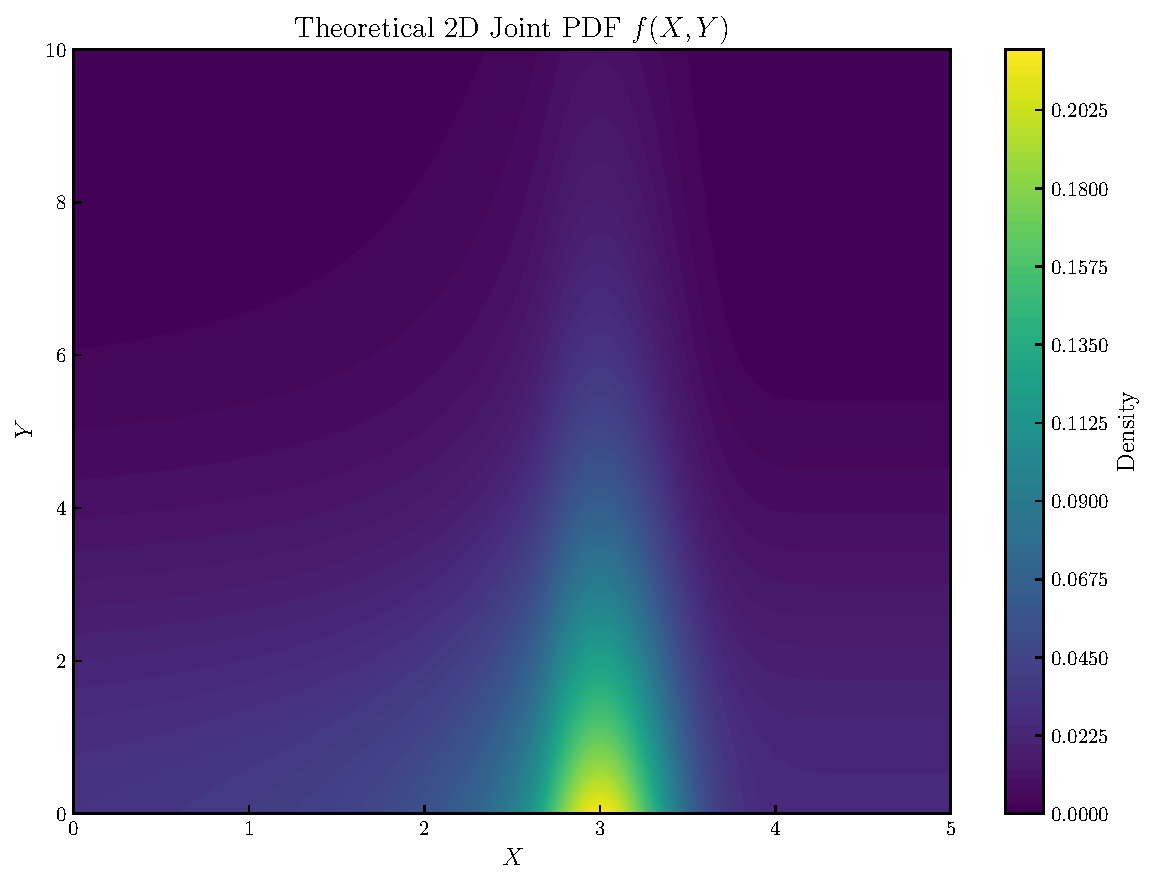
\includegraphics[width=\textwidth, height=0.85\textwidth]{theoretical_joint_pdf.pdf}
        \caption{Theoretical joint PDF of \( X \) and \( Y \).}
        \label{fig:joint_pdf_theoretical}
    \end{subfigure}
    \hfill
    \begin{subfigure}[b]{0.47\textwidth}
        \centering
        \includegraphics[width=\textwidth, height=0.85\textwidth]{output1.png}
        \caption{2D binned joint distribution of sampled data.}
        \label{fig:joint_pdf_sampled}
    \end{subfigure}
    \caption{Comparison between the theoretical joint PDF and the binned joint distribution of sampled data.}
    \label{fig:joint_pdf}
\end{figure}


\begin{figure}[H]
    \centering
    \begin{subfigure}[b]{0.47\textwidth}
        \centering
        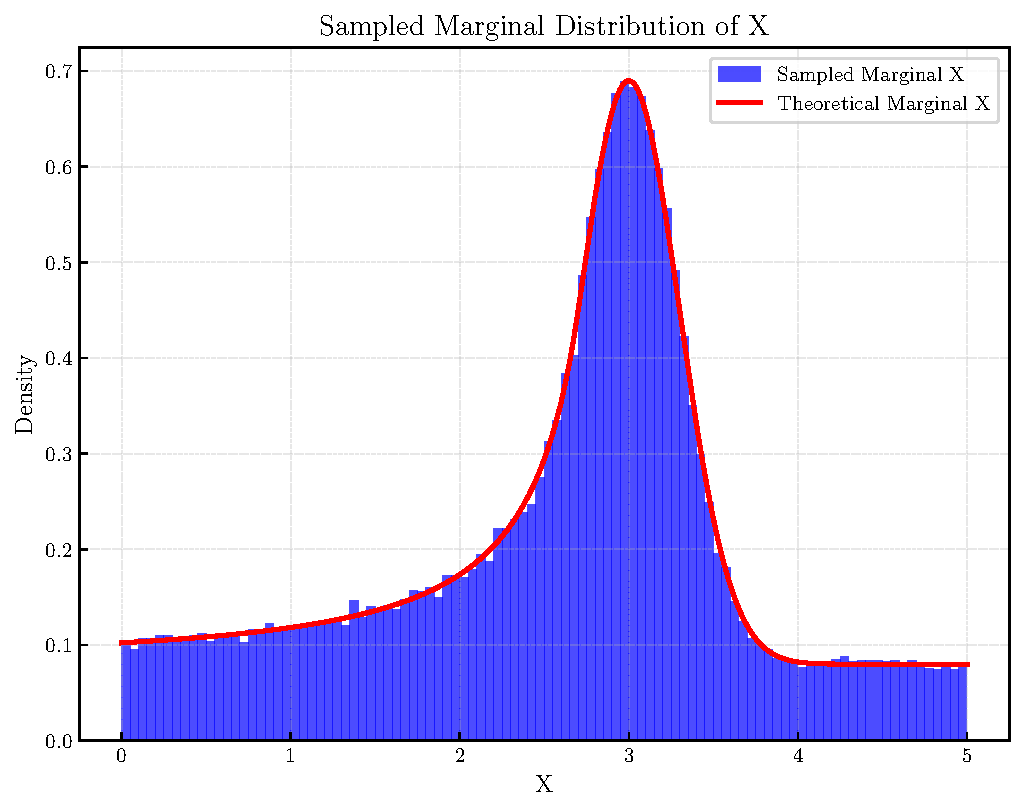
\includegraphics[width=\textwidth, height=0.85\textwidth]{sampled_marginal_X.pdf}
        \caption{Actual and sampled marginal distributions for \( X \).}
        \label{fig:sampled_marginal_X}
    \end{subfigure}
    \hfill
    \begin{subfigure}[b]{0.47\textwidth}
        \centering
        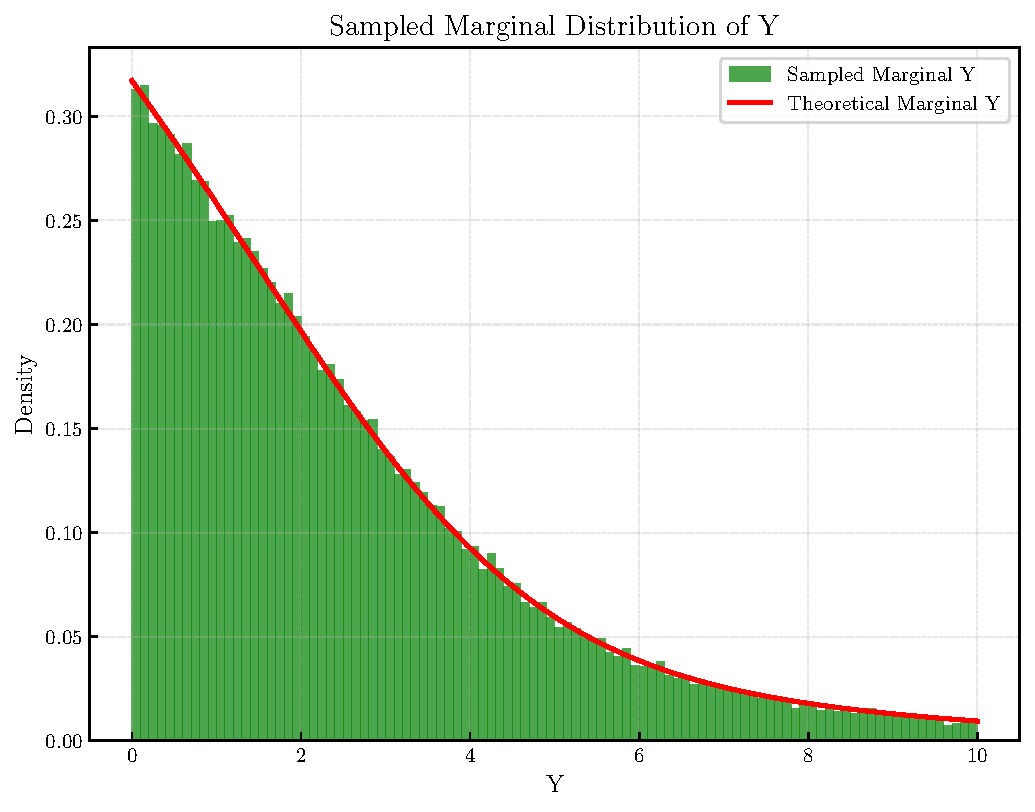
\includegraphics[width=\textwidth, height=0.85\textwidth]{sampled_marginal_Y.pdf}
        \caption{Actual and sampled marginal distributions for \( Y \).}
        \label{fig:sampled_marginal_Y}
    \end{subfigure}
    \caption{Comparison of actual and sampled marginal distributions for \( X \) and \( Y \).}
    \label{fig:marginal_sampling}
\end{figure}



\subsection{Fitting Techniques}
The parameter estimation focuses on extracting the signal parameter \(\lambda\), which defines the exponential decay of the signal in \( Y \). Two distinct methodologies are employed: a joint extended likelihood fit and a weighted fit using \textit{sWeights}. These approaches are detailed below.

\subsubsection{Joint Extended Likelihood Fit}

The joint extended likelihood fit accounts for both the observed number of samples and the probability density of each sample. The primary objective is to estimate \(\lambda\) while simultaneously fitting all other parameters in the joint PDF. The derivation of the likelihood function is as follows~\cite{wakefield2013bayesian}:
\paragraph{Extended Likelihood Function}
The likelihood function for a dataset of \( N_{\text{obs}} \) samples is:
\[
    \mathcal{L} = P(N_{\text{obs}} | N_{\text{exp}}) \cdot \prod_{i=1}^{N_{\text{obs}}} f(X_i, Y_i; \theta),
\]
where:
\begin{itemize}
    \item \( P(N_{\text{obs}} | N_{\text{exp}}) \) is the Poisson probability of observing \( N_{\text{obs}} \) samples given an expected number \( N_{\text{exp}} \),
    \item \( f(X_i, Y_i; \theta) \) is the joint PDF evaluated at the \( i \)-th sample point, and
    \item \( \theta \) represents the set of model parameters, including \(\lambda\).
\end{itemize}

\paragraph{Poisson Contribution}
The Poisson term is expressed as:
\begin{equation}
    P(N_{\text{obs}} | N_{\text{exp}}) = \frac{N_{\text{exp}}^{N_{\text{obs}}} e^{-N_{\text{exp}}}}{N_{\text{obs}}!}.
    \label{eq:poisson_term}
\end{equation}

\paragraph{Extended Log-Likelihood}
Taking the natural logarithm of the likelihood function yields:
\begin{align}
    \ln \mathcal{L} &= \ln P(N_{\text{obs}} | N_{\text{exp}}) + \sum_{i=1}^{N_{\text{obs}}} \ln f(X_i, Y_i; \theta), \\
    &= -N_{\text{exp}} + N_{\text{obs}} \ln N_{\text{exp}} - \ln(N_{\text{obs}}!) + \sum_{i=1}^{N_{\text{obs}}} \ln f(X_i, Y_i; \theta). \label{eq:log_likelihood}
\end{align}
The term \( \ln(N_{\text{obs}}!) \) is constant for a given dataset and does not affect optimization, so it is ignored.

\paragraph{Extended Negative Log-Likelihood}
The extended negative log-likelihood, minimized to extract \(\lambda\) and other parameters, is therefore:
\begin{equation}
    -\ln \mathcal{L} = -N_{\text{obs}} \ln N_{\text{exp}} + N_{\text{exp}} - \sum_{i=1}^{N_{\text{obs}}} \ln f(X_i, Y_i; \theta).
    \label{eq:neg_log_likelihood}
\end{equation}

\paragraph{Implementation Details}
Key aspects of the implementation include:
\begin{itemize}
    \item \textbf{Precomputed Truncation Normalization:} The truncation normalization constant for \( g_s(X) \) is precomputed during each iteration to reduce computational overhead.
    \item \textbf{Numerical Stability:} A small offset (\( 10^{-10} \)) is added to avoid log(0) errors.

\end{itemize}

\begin{itemize}
\item \textbf{Optimization:} The \texttt{iminuit} library is used for optimization~\cite{dembinski2021iminuit}. It employs the MIGRAD algorithm, which minimizes the negative log-likelihood by iteratively updating parameters along the direction of steepest descent. MIGRAD dynamically adjusts step sizes and leverages second-order derivative approximations for efficient convergence. Two uncertainty estimation methods are provided:
\end{itemize}

\begin{itemize}
    \item \textbf{HESSE:} Approximates the covariance matrix by inverting the Hessian matrix at the minimum, providing symmetric uncertainties under the assumption of a quadratic likelihood surface.
    \item \textbf{MINOS:} Computes asymmetric uncertainties by scanning the likelihood function along parameter directions, accounting for non-quadratic behavior near the minimum.
\end{itemize}
HESSE is chosen for its computational efficiency and sufficient accuracy given the well-behaved nature of the likelihood surface in this analysis.


\paragraph{Bounds and Initial Guesses for the Fitting Procedure}


To ensure convergence and accurate parameter estimation during the fitting procedure, we selected \textbf{bounds} and \textbf{initial guesses} for each parameter based on the behavior of the marginal distributions in \(X\) and \(Y\), as shown in Figure~\ref{fig:marginal_sampling}.

\begin{itemize}
    \item \textbf{Parameter \( \mu \) (mean of the signal distribution):} The peak of the signal component \( g_s(X) \) in Figure~\ref{fig:sampled_marginal_X} suggests a location close to \( \mu = 3.0 \). We set the bounds \([2.8, 3.2]\) to focus the fit around this region and chose an initial guess of \( \mu = 3.2 \).

    \item \textbf{Parameter \( \sigma \) (width of the signal distribution):} The signal distribution is relatively narrow, as observed in Figure~\ref{fig:sampled_marginal_X}. Hence, the bounds for \( \sigma \) are set to \([0.05, 0.5]\), with an initial guess of \( \sigma = 0.2 \).

    \item \textbf{Parameter \( \beta \) and \( m \) (shape parameters for the Crystal Ball distribution):} To allow flexibility in modeling the tail of \( g_s(X) \), the bounds are chosen as \(\beta \in [0.5, 1.5]\) and \(m \in [1.0, 2.0]\). The initial guesses of \( \beta = 1.2 \) and \( m = 1.2 \) are close to standard values observed in signal modeling.

    \item \textbf{Parameter \( \lambda_s \) (decay rate for the signal in \(Y\)):} The exponential decay observed in Figure~\ref{fig:sampled_marginal_Y} motivated bounds of \( \lambda_s \in [0.1, 1.0] \), with an initial guess of \( \lambda_s = 0.5 \).

    \item \textbf{Parameters \( \mu_b \) and \( \sigma_b \) (background components):} The background distribution \( g_b(X) \) in Figure~\ref{fig:sampled_marginal_X} and \( h_b(Y) \) in Figure~\ref{fig:sampled_marginal_Y} are flatter and broader. To capture this, we set \( \mu_b \in [-1, 1] \) and \( \sigma_b \in [2.0, 4.0] \), with initial guesses of \( \mu_b = 0.3 \) and \( \sigma_b = 2.7 \).

    \item \textbf{Parameter \( f_{{signal}} \) (signal fraction):} An approximate signal-background balance in the distributions suggested \( f_{\text{signal}} \in [0.1, 0.9] \), with an initial guess of \( f_{\text{signal}} = 0.5 \).

    \item \textbf{Parameter \( N_{{expected}} \) (expected number of events):}  
To account for Poisson fluctuations, the nominal sample size \( N \) is replaced by \( N_{\text{Poisson}} \), a Poisson random variable with mean \( N \). The bounds are then set as:  
\[
N_{\text{expected}} \in [0.75 \cdot N_{\text{Poisson}}, 1.25 \cdot N_{\text{Poisson}}],
\]
with an initial guess of \( N_{\text{expected}} = N_{\text{Poisson}} \).

\end{itemize}




\subsubsection{Weighted Fit Using \textit{sWeights}}


The \textit{sWeights} methodology~\cite{dembinski2022custom} decouples the fitting process into two stages to isolate the signal component in \( Y \) and estimate the decay constant \( \lambda \). The steps are as follows:

\paragraph{Step 1: Fit in \(X\)}The goal of this step is to estimate the signal fraction \( f_{\text{signal}} \) and calculate the signal/background weights (\textit{sWeights}) for each sample \( X_i \). The marginal distribution in \( X \), \( f(X) \), is modeled as a mixture of signal and background components:
\[
f(X_i) = f_{\text{signal}} \, g_s(X_i) + (1 - f_{\text{signal}}) \, g_b(X_i),
\]
where \( g_s(X) \) is the signal PDF and \( g_b(X) \) is the background PDF.

The weights are defined as:
\begin{align}
    w_{\text{signal},i} &= \frac{f_{\text{signal}} \, g_s(X_i)}{f(X_i)}, \label{eq:sweight_signal} \\
    w_{\text{background},i} &= \frac{(1 - f_{\text{signal}}) \, g_b(X_i)}{f(X_i)}. \label{eq:sweight_background}
\end{align}

The parameters of \( f(X) \), including \( \mu, \sigma, \beta, m, f_{\text{signal}}, N_{\text{expected}} \), are estimated using the \texttt{iminuit} library by minimizing the extended negative log-likelihood:
\begin{equation}
    -\ln \mathcal{L}_X = N_{\text{expected}} - N_{\text{Poisson}} \ln(N_{\text{expected}}) - \sum_{i=1}^{N_{\text{Poisson}}} \ln \left[ f_{\text{signal}} g_s(X_i) + (1 - f_{\text{signal}}) g_b(X_i) \right].
\end{equation}

This fit allows us to determine the signal fraction \( f_{\text{signal}} \) and extract of the signal weights \( w_{\text{signal},i} \), which are used to isolate the signal contribution in \( Y \).

\paragraph{Step 2: Weighted Fit in \( Y \)}  
The signal weights \( w_{\text{signal},i} \) obtained from Step 1 are used to isolate the signal component and perform a weighted fit on the marginal distribution in \( Y \) to estimate \( \lambda \). The weighted likelihood function in \( Y \) is:
\begin{equation}
    \mathcal{L}_Y = \prod_{i=1}^{N_{\text{Poisson}}} h_s(Y_i)^{w_{\text{signal},i}},
\end{equation}
where \( h_s(Y) \) is the signal PDF in \( Y \).

Taking the negative logarithm gives the weighted log-likelihood:
\begin{equation}
    -\ln \mathcal{L}_Y = -\sum_{i=1}^{N_{\text{Poisson}}} w_{\text{signal},i} \ln h_s(Y_i).
\end{equation}

The parameter \( \lambda \) is extracted by minimizing this weighted negative log-likelihood using the \texttt{iminuit} library.



\section{Computational Efficiency Benchmarking}

To evaluate the computational performance of our implementation, we benchmarked three main tasks:
\begin{enumerate}
    \item \textbf{Random Sampling from a Normal Distribution:} Using \texttt{np.random.normal} as a baseline.
    \item \textbf{Sample Generation:} Generating samples from the combined signal and background distributions using the defined methods.
    \item \textbf{Fitting:} Performing the extended likelihood fit using the generated samples.
\end{enumerate}

The benchmarking was conducted for a dataset of \( 100,000 \) samples, averaged over \( 100 \) repetitions. The results include average execution times, standard deviation of execution times, and relative times compared to \texttt{np.random.normal}.

\begin{table}[H]
    \centering
    \caption{Benchmarking Results for Sampling and Fitting Techniques}
    \label{tab:benchmark}
    \begin{tabular}{|l|c|c|c|}
        \hline
        \textbf{Task} & \textbf{Average Time (s)} & \textbf{Std Dev (s)} & \textbf{Relative Time} \\ \hline
        \texttt{np.random.normal} (Baseline) & \( 0.001797 \) & \( 0.000930 \) & \( 1.000 \) \\ \hline
        Joint PDF Sampling & \( 0.009922 \) & \( 0.001255 \) & \( 5.521 \) \\ \hline
        Maximum Likelihood Fit & \( 1.755148 \) & \( 0.023208 \) & \( 976.622 \) \\ \hline
    \end{tabular}
\end{table}

The results indicate that:
\begin{itemize}
    \item \textbf{Sampling} is approximately \( 5.5 \) times slower than baseline normal sampling. This is due to the added complexity of sampling from non-standard distributions (e.g., truncated Crystal Ball and exponential distributions), which require numerical techniques such as CDF construction, interpolation, and inversion instead of direct sampling.
    \item \textbf{Maximum likelihood fitting} is significantly more computationally intensive, with a relative time of approximately \( 977 \) times the baseline. This is because the likelihood fit relies on iterative optimization using numerical methods. In the absence of analytic gradients, MIGRAD estimates gradient vectors numerically using finite differences by perturbing each parameter slightly and recalculating the negative log-likelihood across the entire dataset. Computing this negative log likelihood each time to calculate each partial derivative making up the gradient vector, per optimization iteration, until convergences is extremely costly. Additionally, MIGRAD dynamically approximates second-order derivatives (Hessian elements) to optimize step size and convergence, further increasing computational cost.
    
\end{itemize}

\section{Bootstrapping Analysis}

Bootstrapping is utilized to evaluate the performance of the two fitting methodologies—joint extended likelihood fit and \textit{sWeights} fit—in estimating the decay constant \(\lambda\). This involves generating multiple trials over varying sample sizes, performing fits for each trial using each method, and analyzing the resulting uncertainties and biases, along with the errors associated with these metrics.

\subsection{Methodology}

The bootstrapping procedure follows these steps:

\begin{enumerate}
    \item \textbf{Generate Bootstrap Samples:} For each trial, synthetic datasets are generated using the sampling techniques described earlier. Sample sizes range from \(500\) to \(10000\) to evaluate scaling behavior.
    
    \item \textbf{Perform Fits:} Each synthetic dataset is fitted using both the joint extended likelihood fit and the \textit{sWeights} fit to extract the decay constant \(\lambda\).

    \item \textbf{Repeat:} The process is repeated for \(N_{\text{trials}} = 250\) bootstrap trials per sample size to ensure statistical robustness.

    \item \textbf{Calculate Metrics:}
    \begin{itemize}
        \item \textbf{Bias:} The bias in the fitted decay constant \(\lambda\) is defined as:
        \begin{equation}
        \text{Bias} \; (\delta_{\lambda}) = \langle \hat{\lambda} \rangle - \lambda_{\text{true}},
        \label{eq:bias_definition}
        \end{equation}
        where \( \langle \hat{\lambda} \rangle = \frac{1}{N} \sum_{i=1}^{N} \hat{\lambda}_i \) is the mean of the fitted decay constants across all trials, and \( \lambda_{\text{true}} \) is the true value of the decay constant.

        \item \textbf{Uncertainty:} The uncertainty \(\sigma_{\lambda}\) in the fitted decay constant is given by the standard deviation of the fitted values:
        \begin{equation}
        \sigma_{\lambda} = \sqrt{\frac{1}{N-1} \sum_{i=1}^{N} \left( \hat{\lambda}_i - \langle \hat{\lambda} \rangle \right)^2},
        \label{eq:uncertainty}
        \end{equation}
        where \(N\) is the number of bootstrap trials, and \(\hat{\lambda}_i\) is the fitted decay constant from the \(i\)-th trial.

        \item \textbf{Bias Error:} The error on the bias \(\Delta_{\delta_{\lambda}}\) reflects the statistical uncertainty in estimating the mean of the fitted decay constants \(\langle \hat{\lambda} \rangle\). This is derived as:
        \begin{equation}
        \Delta_{\delta_{\lambda}} = \frac{\sigma_{\lambda}}{\sqrt{N}},
        \label{eq:bias_error}
        \end{equation}
        where \(\sigma_{\lambda}\) is the standard deviation of the fitted values, and \(\sqrt{N}\) arises because the mean is estimated from \(N\) independent trials.

        \item \textbf{Uncertainty Error:} The error on the uncertainty \(\Delta_{\sigma_{\lambda}}\) quantifies the uncertainty in the estimation of the standard deviation \(\sigma_{\lambda}\). Using propagation of error and the variance of the sample variance, it is given by:
        \begin{equation}
        \Delta_{\sigma_{\lambda}} = \frac{\sigma_{\lambda}}{\sqrt{2(N-1)}}.
        \label{eq:uncertainty_error}
        \end{equation}
        This expression is derived from the asymptotic variance of the sample standard deviation. 
    \end{itemize}
\end{enumerate}


The results of the bootstrapping analysis are presented below. Figure~\ref{fig:bias_vs_sample_size} illustrates the bias in the fitted decay constant \(\lambda\), while Figure~\ref{fig:uncertainty_vs_sample_size} shows the uncertainties as a function of sample size.

\begin{figure}[H]
    \centering
    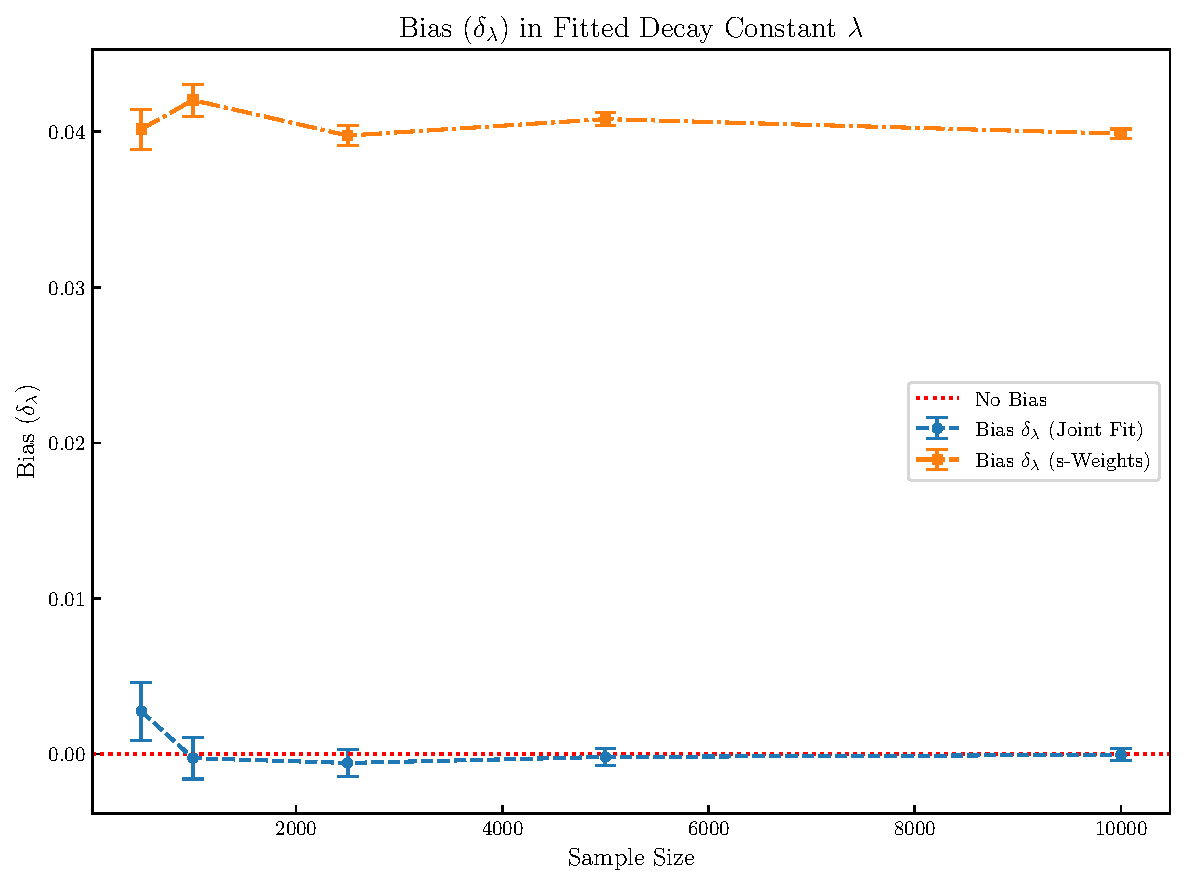
\includegraphics[width=0.8\textwidth]{Combined_Bias_with_ErrorBars.pdf}
    \caption{Bias \(\delta_{\lambda}\) in the fitted decay constant \(\lambda\) as a function of sample size. The joint extended likelihood fit exhibits negligable bias \((\delta_{\lambda} \approx 0)\), whereas \textit{sWeights} method shows a constant bias of approximately \( \delta_{\lambda} \approx 0.04 \) across the sample sizes}
    \label{fig:bias_vs_sample_size}
\end{figure}

\begin{figure}[H]
    \centering
    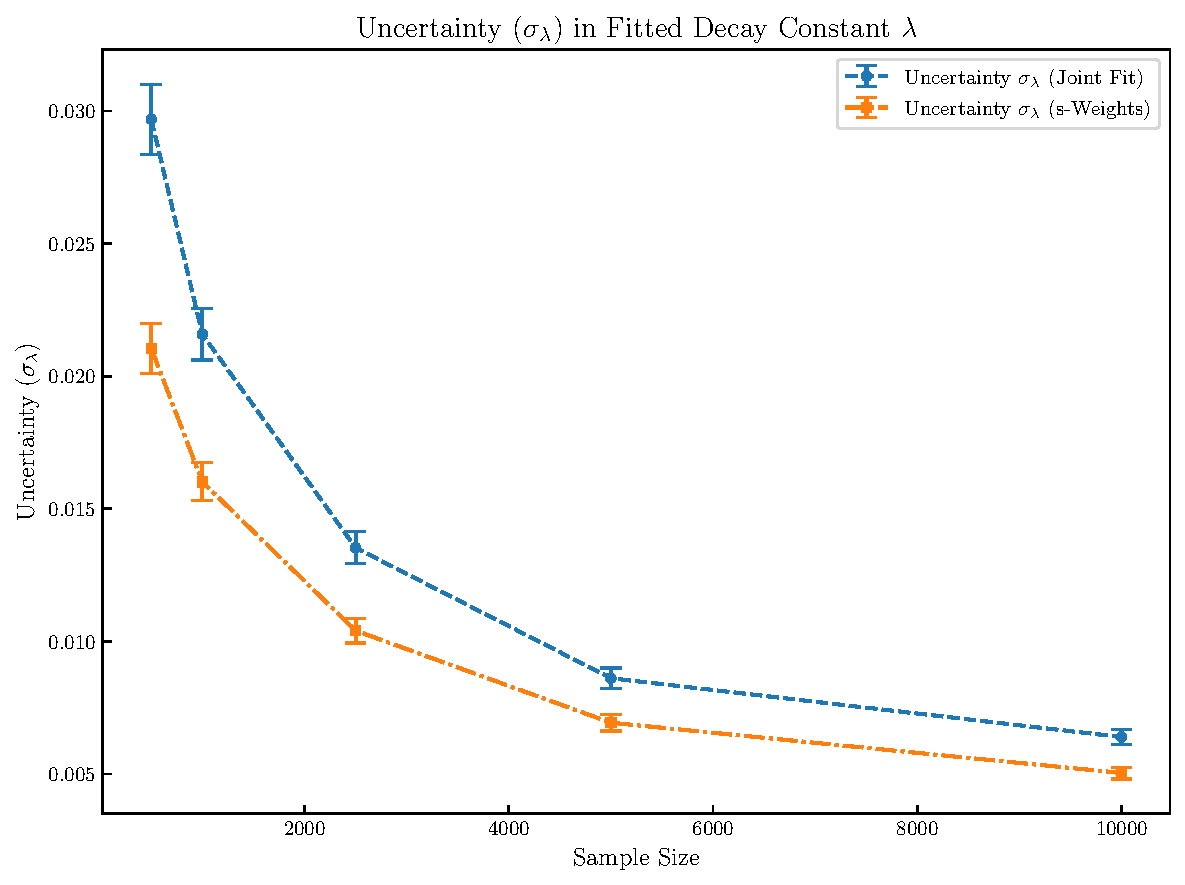
\includegraphics[width=0.8\textwidth]{Combined_Uncertainty_with_ErrorBars.pdf}
    \caption{Uncertainty \(\sigma_{\lambda}\) in the fitted decay constant \(\lambda\) as a function of sample size. Both methods show decreasing uncertainties with increasing sample size, but the joint extended likelihood fit has consistently higher uncertainties compared to the \textit{sWeights} method.}
    \label{fig:uncertainty_vs_sample_size}
\end{figure}


\subsection{Discussion}

\paragraph{Bias:}  
The joint extended likelihood fit exhibits negligible bias in the fitted decay constant \(\lambda\), while the \textit{sWeights} method shows a small but persistent bias of approximately \( \delta_{\lambda} \sim 0.04 \) across all sample sizes. This behavior arises due to fundamental differences in how the two methods utilize the full joint distribution \( f(X, Y) \) and handle correlations between the variables \( X \) and \( Y \):

\begin{itemize}
    \item \textbf{Joint Fit:}  
    The joint extended likelihood fit models the signal and background components simultaneously within a single optimization framework, using the full joint PDF \( f(X, Y) \). By explicitly accounting for correlations between \( X \) and \( Y \), this method avoids structural assumptions and achieves an unbiased estimation of \(\lambda\). As the sample size increases, statistical fluctuations diminish due to averaging, further reducing the bias.
    
\item \textbf{\textit{sWeights} Fit:}  
The signal weights \( w_{\text{signal},i} \) are calculated from a marginal fit in \( X \), which estimates the signal fraction \( f \) from the marginal PDFs \( g_s(X) \) and \( g_b(X) \). In practice, finite sample sizes, imperfect bounds and initial guesses can lead to incorrect and local instead of global convergences during the fit introducing statistical uncertainties and inaccuracies in these estimates. These uncertainties propagate into the signal weights, such that they are imperfect representations of the true signal contribution. When these imperfect weights are applied in the weighted fit in \( Y \), the reconstructed signal distribution does not perfectly isolate \( h_s(Y) \), introducing a systematic bias in the parameter estimation.





\end{itemize}
\paragraph{Uncertainty:}  
The uncertainties \(\sigma_{\lambda}\) in the fitted decay constant decrease as a function of the sample size \( N \), as expected. The uncertainties scale as:
\[
\sigma_{\lambda} \propto \frac{1}{\sqrt{N}},
\]
where \( N \) is the number of samples in the dataset. This behavior arises because parameter estimates rely on the statistical information contained in the data. By the \textit{Central Limit Theorem} (CLT), the standard error of an estimated parameter decreases inversely with the square root of the number of independent observations \( N \). The intuition behind this is that larger sample sizes lead to more accurate estimations of the parameter, reducing the standard deviation of the distribution of the fitted parameter obtained from the trials.

In figure~\ref{fig:uncertainty_vs_sample_size}, the joint fit consistently shows slightly larger uncertainties compared to the \textit{sWeights} fit. This difference likely arises because the joint fit involves simultaneous optimization over multiple parameters, introducing additional variability, whereas the \textit{sWeights} method performs a simpler weighted fit.
\subsection{Comparison of the Joint Fit and \textit{sWeights} Methods}

The joint extended likelihood fit and the \textit{sWeights} method offer different trade-offs between accuracy and efficiency:

\begin{itemize}
    \item \textbf{Joint Fit:} Provides unbiased parameter estimates by simultaneously fitting the signal and background components, accounting for correlations between \( X \) and \( Y \). However, it is computationally intensive due to the simultaneous optimization of multiple parameters.
    
    \item \textbf{\textit{sWeights} Fit:} Computationally efficient and well-suited for large datasets where marginal signal and background models in \( X \) are accurately known and can be well fitted. However, it assumes no correlations between \( X \) and \( Y \) in the joint PDF, leading to systematic biases if this assumption is violated.
\end{itemize}

In practice, the joint fit is preferred for precision analyses where correlations and model imperfections are critical, while the \textit{sWeights} method is advantageous for exploratory studies or when computational resources are limited.
\section{Conclusion}

In this study, we compared the joint extended likelihood fit and the \textit{sWeights} method for estimating the decay constant \(\lambda\). The joint fit, while computationally intensive, provided unbiased estimates and accounted for correlations between variables \(X\) and \(Y\). In contrast, the \textit{sWeights} method, though computationally efficient, introduced a small systematic bias due to its decoupling of the fits. The results show that the joint fit is ideal for precision-focused tasks, whereas the \textit{sWeights} method is more suitable for large datasets or computationally constrained scenarios.


\newpage
% Bibliography
\bibliographystyle{unsrt}
\bibliography{references} % Ensure you have a .bib file named "references.bib" in your working directory



% Appendix Section
\appendix
\section*{Appendix}
\addcontentsline{toc}{section}{Appendix}

\section{Declaration of Autogenerative Tools}

In this project, I used GitHub Copilot as a coding assistant. I mainly used it to generate the plots in part c), the table in d), and the bias and variance plots in part e) and f). I also used it within my code to create comments, docstring my functions, debug and format markdown cells explaining the different sections in the notebook.

In regards to the report, I used the Overleaf AI which uses ChatGPT to help write the mathematics in latex format, and also used it to correctly format various sections of the report as I am quite new to LaTeX.

\end{document}